\subsection{Ampersand as method} \label{Ampersand as method}
\def\cat{2}
The way of working with Ampersand requires preparation in the design and structuring of the work.
Experience plays a major role in this.
In the section on useful (see~\ref{useful}) it was pointed out to maintain overview.
Keeping an overview helps when there are agreements about the naming of the Concepts, Relations and Rules.

\begin{table}[H]
    \begin{tabularx}{\linewidth}{|X|X|}
        \hline
        Category        & CAT1-\cat \\\hline
        Category Title  & \acrshort{cat\cat} \\\hline
        Definition      & \acrlong{cat\cat} \\\hline
        Anchor examples & 
        \begin{itemize}
        \setlength{\itemindent}{-2em}
            \item rq1-25:12-9: First make an overview of all laws and regulations.
            \item rq1-80:20-11: A consistent naming of a concept is necessary.
        \end{itemize}
        \\\hline
        Coding rules    & Approach and working with Ampersand \\\hline
    \end{tabularx}
    \caption{Category \acrshort{cat\cat}}
    \label{tab:Ampersand as method}
\end{table}

Naming conventions to have these consistent in the scripts and therefore in the Conceptual design are important for readability.
Also, working with Includes and Patterns to obtain small delineated pieces of functionality is important for the overview.
The agreements are also necessary to find concepts and relationships in the scripting.

In order to maintain an overview of the relations, an Excel sheet was drawn up in which the relations could be compiled.
This was to have support in the allocation of the multiplicities.
And was it possible to copy the relation definition to a script.
\begin{figure}[H]
    \centering
    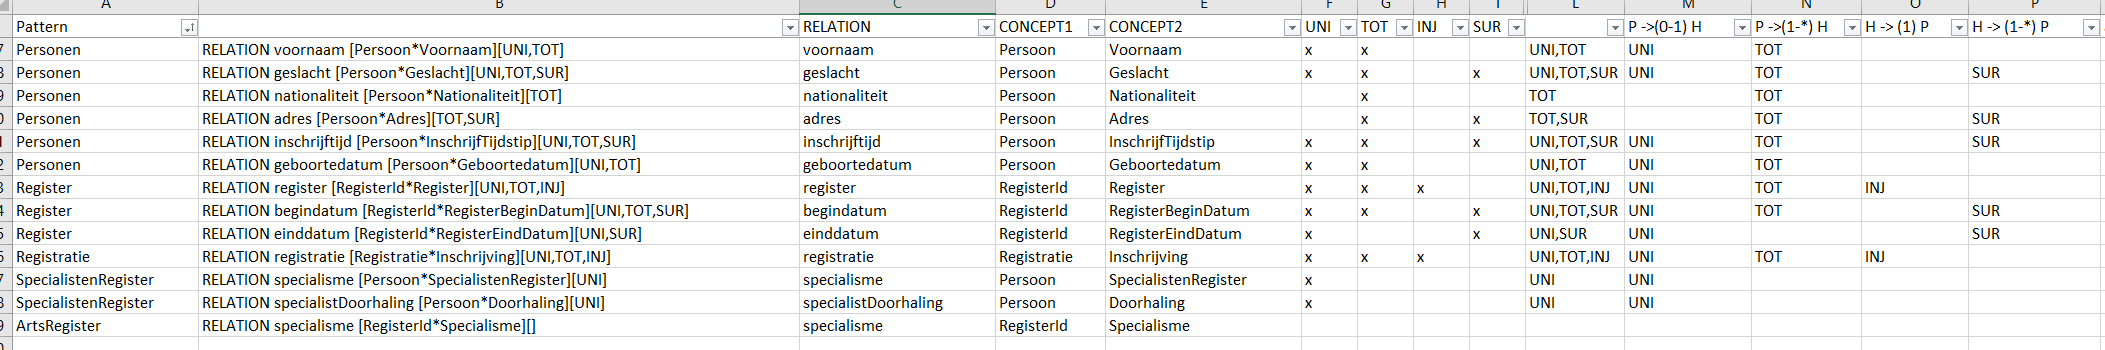
\includegraphics[width=1\textwidth]{excel relatie overzicht.PNG}
    \caption{excel relation overview}
    \label{fig:excel relation overview}
\end{figure}

The method Ampersand uses involves applying Rules to Relationships.
Conceptually, the Rules are easy to define, but physically difficult to implement.
It requires knowledge of Relation algebra to be able to work with this correctly.
And it requires knowledge of Ampersand because it requires a certain way of notation.
In the appendix \ref{appendixAdl} are examples of how to use Rules.

The method allows multiple uses of the same Concepts and Relations.
This is only visible when the documentation is generated.
By allowing the Concepts and Relationships multiple times, it is possible to add different definitions to them.

In addition to the technical approach, there is also a working method in which the user is involved.
In this case, it is important that a lawyer is involved at the start of the work.
Because Ampersand's approach to the definition is not very technical, a lawyer can easily understand this.
An analyst, as mentioned earlier, can perform this together with a lawyer

Validation of the data uses a prototype and conceptual design.
This has not been substantively validated, because then it is only checked whether the laws and regulations are well understood.
Extremely important for a system, but not for this study.
The Conceptual design was labeled as understandable, recognizable and useful.
The prototype was viewed through ICT glasses.
It has been noted that it does not meet the \acrshort{cibg} requirements for a website.
This is usually not a problem for an IT employee, but a user usually also looks at the design.
It has been indicated that this is possible through a CSS adjustment, but how exactly this should be done is not entirely clear.

The recognition of Ampersand as instigator of real time signal violations is not reflected in the interviews.

